\documentclass[american, oneside]{ecsgdp}
\usepackage[utf8]{inputenc}

% packages
\usepackage[capitalise]{cleveref} % auto format cross-references
\usepackage{svg} % SVG file compatibility
\usepackage{babel} % dependency of BibLaTeX
\usepackage{csquotes} % dependency of BibLaTeX
% \usepackage[style=plain, backend=biber]{biblatex} % for citing
\usepackage{natbib}
% \addbibresource{Latex/refs.bib}


\graphicspath{{img/}}

\begin{document}

\frontmatter
\title{Thesis Proposal}
\authors{Gonem Lau}
\addresses{\groupname\\\deptname\\\univname}
\date{\today}
\keywords{restaurant reviews, semantic web, sentiment analysis, natural language processing, machine learning, neural network, unsupervised learning}
\logo{logo_eur.eps}{1.75in}

% \include{digital-version}

\maketitle

\tableofcontents

\mainmatter
%%%%%%%%%%%%%%%%%%%%%%%%%%%%%%%%%%%%%%%%%%%%%%%%%%%%%%%%%%%%%%%%
\chapter{Introduction} \label{chap:introduction}
This chapter presents the topic, motivations and goals of this paper. \cref{sec:problem} introduces the problem of Aspect-Based Sentiment Analysis and explains the motivations of this field. Next, \cref{sec:objective} describes the objectives of the the work and its novelties. Last, \cref{sec:structure} presents the structure of the remaining chapters. % List of Abbreviations?

\section{Problem Statement} \label{sec:problem}
With virtually everyone having access to the Web, it is not unthinkable that tons of texts could be written every second of everyday. With all that content being generated by users, it is not feasible to manually analyze all texts. Therefore, many methods in the field of Natural Language Processing have been proposed to extract information from these textual data. One interesting subfield, Sentiment Analysis, is to discover and understand opinions from user-generated data \parencite{Liu2012SAOP}. For example, companies can improve their products or services after analyzing customer sentiments from reviews. Not only businesses profit from this field, customers benefit too. Customers can find products more easily that are up to their standards.

With Sentiment Analysis, one could analyze the text on different levels: document-level, sentence-level, or aspect-level \parencite{Liu2012SAOP}. The distinction exists because a review (document) or even a sentence could contain multiple sentiments addressing multiple aspects. For example, \cref{fig:example_review} considers a reviewer that had a positive sentiment towards the food while being more negative towards the interior.

\begin{figure}[htbp]
  \centering
  \includesvg{example_review.svg}
  \caption{An illustrative example of ABSA subtasks.}
  \label{fig:example_review}
\end{figure}

This paper focuses on Aspect-Based Sentiment Analysis (ABSA), which mainly aims to extract all aspects of a product or service mentioned in a review, and classify the sentiment for each aspect \parencite{Liu2012SAOP}. However, the task is not strictly bounded. For example, some datasets provide the aspect category whereas others provide targets, in which targets are the explicit aspect expressions found in a sentence. Sentiment classification can also differ per dataset. For example, the SemEval datasets provided by \textcite{Pontiki2015SemEval, Pontiki2016SemEval} define sentiment as positive, neutral, or negative. While the Yelp2014 dataset \parencite{Tang2016Yelp} ranks sentiment on a 5 star range.

In more detail, the target could be described with one or multiple aspect categories, and optionally with the aspect term(s). While sentiment could be described with the sentiment polarity and optionally with the opinion term(s). Therefore, ABSA research could be divided into four subtasks: Aspect Term Extraction (ATE), Aspect Category Detection (ACD), Opinion Term Extraction (OTE), and Aspect Sentiment Classification (ASC) \parencite{Zhang2022Survey}. ATE aims to extract explicit aspect expressions within a given text. ACD categorizes the aspects into a predefined set of categories. OTE extracts explicit opinion terms towards aspects. ASC predicts the sentiment polarity for each aspect within a sentence. To illustrate these tasks with the previous example in \cref{fig:example_review}, ATE extracts the explicit terms ``food'' and ``interior''. ACD categorizes the targets to \texttt{FOOD\#QUALITY} and \texttt{AMBIENCE\#GENERAL}, respectively. OTE, extracts the explicit terms ``Excellent'' and ``could use some help''. ASC predicts the aspects to be positive and negative, respectively. The main focus of this research is Aspect Category Sentiment Detection (ACSD), which contains three compound tasks found in ABSA: ATE, ACD, and ASC. Therefore, the OTE task will not be investigated.

\section{Research Objective} \label{sec:objective}
ABSA solutions can be classified in three different types: rule-based methods, supervised machine-learning and unsupervised machine-learning \parencite{Schouten2016Survey}. In the beginning, rule-based approaches were investigated such as the model proposed by \textcite{Hu2004Rules}. However, with more access to computational power, machine learning and especially neural models have been growing in popularity as seen when comparing by the earliest survey by \textcite{Schouten2016Survey} and a more recent survey by \textcite{Zhang2022Survey}. Rule-based approaches felt out of favor as they required careful constructions which involve lots of manual effort. Yet, some models exploit both approaches with great results \parencite{Trusca2020HAABSA++, Meskele2020ALDONAr}. Until recently, the majority of the machine-learning approaches focuses on supervised models which yield great results \parencite{Zhang2022Survey}. However, supervised approaches require large datasets which take substantial effort to construct, especially on aspect level. Therefore, un- or semi-supervised models are one of the ways that have been devised to overcome the struggles presented by previous approaches \parencite{He2017ABAE}. Unsupervised models show great potential as their performance itches closer and closer to supervised methods.

As stated above, the field of ABSA is not confined to a single task. Nevertheless, most methods address a single subtask rather than multiple. For example, the sophisticated supervised LCR-Rot-hop++ \parencite{Trusca2020HAABSA++} model exploits the position of the target. Therefore, the data would have to include the explicit aspect expression, or ATE has to be performed beforehand. Yet, some efforts have been made to create a compound solution by considering a set of inter-related dependencies from the four subtasks. One of which is the Aspect category and Sentiment Classification (CASC) \parencite{Kumar2021CASC} model, which is a weakly-supervised approach to the ACD and ASC tasks. CASC follows a three-step process. First, class vocabularies for aspect and sentiment categories are constructed using only seed words. Second, unlabeled data is turned into labeled data in a weakly-supervised manner. Third and last, a compound neural model is implemented to perform ACD and ASC.

The authors of CASC used a simple linear layer in the third step. Therefore, swapping the linear layer with a more sophisticated neural model is unexplored territory. In this paper, we explore injecting LCR-Rot-hop++ \parencite{Trusca2020HAABSA++} into CASC \parencite{Kumar2021CASC}. Furthermore, LCR-Rot-hop++ was originally constructed to only perform ASC. However, we also explore the performance of LCR-Rot-hop++ for ACD. As noted earlier, the second step of CASC is modified to also perform ATE to exploit positional information of aspects. In short, our research question can be summarized as follows:

\begin{center}
    \textit{What is the influence of injecting a sophisticated neural model in a unsupervised framework, and what is the effect of applying a single-task model to a compound one?}
\end{center}

As mentioned above, ABSA is a helpful tool for both businesses and customers. With the help of unsupervised models, businesses do not have to create a large division of their staff to manually go through their reviews. With unsupervised compound ABSA models being relatively unexplored, we propose a novel model which we compare against both supervised and unsupervised models. Second, the model extends the first model to exploit the positional information of the target by replacing the simple model in the three step with a modified LCR-Rot-hop++ model. Comparisons are made using the SemEval dataset challenges \parencite{Pontiki2015SemEval, Pontiki2016SemEval}. In short, our main contributions can be summarized as follows:

\begin{itemize}
    \item We extend CASC by extracting aspect terms during the second step, meaning that performance should not be affected if positional information is not exploited. Meaning that the model is able to perform the ATE task indirectly besides the ACD and ASC tasks.
    \item We adapt and compare the CASC model in step three. The linear layer gets replaced by the sophisticated LCR-Rot-hop++ model. Therefore, positional information gets exploited unlike in the simple linear layer.
    \item We explore the performance effects of LCR-Rot-hop++ for the ACD task. The model is originally performed for ASC only. Therefore, inter-dependent information between ACD and ASC might get exploited by tackling the task in a compound manner.
\end{itemize}

The implementation is based on code provided by \textcite{Kumar2021CASC}. FOR NOW, THE CODE IS DEVELOPED USING THE PYTORCH LIBRARY, BUT I MIGHT DECIDE TO KEEP ON USING TENSORFLOW. ONCE THIS HAS BEEN DECIDED, THIS SECTION WILL CONTAIN A SHORT DESCRIPTION OF THE LIBRARY. The source code for this paper can be found at \url{https://github.com/Gogonemnem/BSc2-thesis-ba-qm}

\section{Thesis Structure} \label{sec:structure}
The paper continues as follows. \cref{chap:related_work} provides an overview of prior approaches proposed in ABSA. Next, \cref{chap:data} illustrates the datasets used in the empirical analysis. Afterwards, the proposed models in this paper are thoroughly explained in \cref{chap:methodology}. In \cref{chap:results}, the performance of the proposed models are compared against other state-of-the-art approaches. Last, main findings are presented in \cref{chap:conclusion} together with some limitations and suggestions for future research.

%%%%%%%%%%%%%%%%%%%%%%%%%%%%%%%%%%%%%%%%%%%%%%%%%%%%%%%%%%%%%%%%
\chapter{Related Work} \label{chap:related_work}
This chapter presents an overview and a review of previous works. First, \cref{sec:paradigms} explains the different paradigms that are often used to solve the ABSA task. Furthermore, it dives into why some paradigms are more compatible with unsupervised methods. Next, \cref{sec:single} explores methods that have been proposed in recent years to solve subtasks in ABSA individually. Afterwards, \cref{sec:compound} shows recent progressions towards solving multiple subtasks in a compound manner. 

\section{Model Paradigms} \label{sec:paradigms}
Before describing the works appearing in ABSA, we briefly explore four common modeling paradigms adopted from NLP: Sequence-level Classification (SeqClass), Token-level Classification (TokenClass), Machine Reading Comprehension (MRC), Sequence-to-Sequence modeling (Seq2Seq).

%!!!!!!!! This paragraph needs a bit more explanation
In SeqClass, input text is usually encoded to extract task-specific features which get used by a classifier to predict the correct label. Next, TokenClass is also known as sequence labeling or sequence tagging, which assigns a label to each token in the input text. In contrast to SeqClass, TokenClass classifies every token within a sequence rather than the sequence itself. For ABSA, it is common to use the BIOES tagging scheme (B-beginning, I-inside, O-outside, E-ending, S-singleton). Then, MRC extracts spans of texts from input text conditionally on a given query. For example, a query could be ``What are the aspect terms?'' which then extracts the start and end position of the text spans corresponding to the aspects. Therefore, MRC does not have to extract the inner tokens unlike TokenClass. Last, Seq2Seq aims to generate an output sequence from an input sequence. For example, this paradigm has been applied to translating texts.

Although the TokenClass paradigm has seen some unsupervised methods, such as in identification of idiomatic expression \parencite{Fazly2009UnsupervisedTokenClass}, ABSA has basically seen no progression for unsupervised the paradigm. The same holds for the MRC and Seq2Seq paradigm. Other fields such as question and answering \parencite{Cui2020UnsupervisedMRC} and translation \parencite{Ramachandran2017UnsupervisedSeq2Seq} has seen some progression. However, ABSA has not seen progression as it is uncommon to use MRC and Seq2Seq methods for ABSA tasks \parencite{Zhang2022Survey}. Therefore, mostly unsupervised SeqClass methods are explored due to the compatibility with ABSA tasks.

\section{Single ABSA Tasks} \label{sec:single}
This section presents different subtasks within ABSA handled as single tasks. However, the OTE task will not be discussed as we do not aim to extract opinion expressions in the compound model. In other words, the following paragraphs present the progressions made in ATE, ACD, and ASC.

\subsection{Aspect Term Extraction (ATE)} \label{sec:ATE}
With ATE aiming to extract the explicit aspect expressions, supervised methods often formulate the subtask as a TokenClass problem. The reason is that usually the aspect expression can be found in the text input.

% \todo{papers from Yin CRF, Liu RNN, Xu CNN}

While supervised approaches yield impressive results, they often require large labeled datasets. The neural models are not bottlenecked by their simplicity but rather by the available data \parencite{Huang2020JASen}, which motivates the latest trend of creating un- and semi-supervised models.  

% \todo{small examples of non-neural solutions?}

Many approaches have been explored but there is no framework that has a clear lead. \textcite{He2017ABAE} propose the Attention-based Aspect Extraction (ABAE) model which de-emphasizes irrelevant words through an attention mechanism to improve the coherence of extracted aspects. \textcite{Liao2019LCC+GBC} propose LCC+GBC, which leverages local and global contexts to extract aspects. Then, \textcite{Tulkens2020CAt} propose CAt, a simple solution in which they only use a Part of Speech (POS) tagger and domain-specific word embeddings to extract aspects using a contrastive attention mechanism. The authors mention that a potential drawback of this method might be its simplicity. Although the model performs well, it might perform worse on more difficult or sophisticated dataset challenges. 
%\todo{mention Shi's paper contrastive framework? I might not employ any contrastive mechanisms}


\subsection{Aspect Category Detection (ACD)} \label{sec:ACD}
With ACD aiming to identify the categories of a sentence or aspect, the SeqClass paradigm is usually applied. One advantage of applying ACD over ATE is that no explicit aspect expressions have to be in the sentence. For example, ``It's expensive and gross'' could be categorized to the \texttt{PRICE} and \texttt{FOOD} categories, whereas ATE can not identify what is being reviewed. Furthermore, ACD predicts the categories jointly, whereas ATE extracts aspects separately, thus losing information. Therefore, supervised methods approach the task as a multi-label assignment problem. 

However, tackling ACD in an unsupervised manner has a different approach. Therefore, supervised methods are not discussed. Unsupervised ACD loses the advantages over ATE mentioned above. The approaches often consist of ATE and, subsequently, single-label ACD on the aspect terms. First, candidate aspect terms, which are likely to be the aspects, are extracted. Then, those candidate terms are mapped or clustered to the pre-defined aspect categories. Please refer to \cref{sec:ATE} for the first ATE step. One of the earlier unsupervised ACD methods was ABAE. One drawback of this model is that the learned aspects need to be mapped manually. Therefore, \textcite{Karamanolakis2019Seed} propose a teacher-student framework that extends the ABAE model by leveraging seed words eliminating the need to manually assigning the learned aspects. % If Shi included, also include here.

\subsection{Aspect Sentiment Classification (ASC)} \label{sec:ASC}
Similar to ACD, ASC is usually implemented with the SeqClass paradigm, labeling each aspect to a polarity score. Although ASC has seen many supervised methods through the years \parencite{Zhang2022Survey}, the single task of ASC has not seen much progression in the field of unsupervised learning. The most likely reason is that input data about aspects are needed to classify sentiment on an aspect level. Input data can be provided in two different ways, aspects provided could be either the aspect term or category. Differences are subtle, but one interesting difference is that positional information can be exploited with aspect term data.

An interesting framework that exploits such positioning is the LCR-Rot model by \textcite{Zheng2018LCR-Rot} which splits sentences in a left context, target, and right context. This model has been extended to exploit lexical reasoning, multiple attention mechanisms and contextual embeddings \parencite{Schouten2017Ontology, Wallaart2019HAABSA, Trusca2020HAABSA++}.

\section{Compound ABSA Tasks} \label{sec:compound}

Models for multiple tasks has seen many variants. This is also because some authors focus on different combinations of different tasks. 

Early studies in unsupervised learning that jointly extract aspect and sentiments are mostly based on Latent Lirichlet Allocation (LDA) \parencite{Blei2003LDA}. \textcite{Xu2012JAS} propose the Joint Aspect/Sentiment model (JAS) which adapts LDA by introducing sentiment-related variables and integrating sentiment prior knowledge. \textcite{Zhao2010MaxEnt-LDA} further extract aspect-specific opinions in a generative process. \textcite{Wang2015Boltzmann} introduced a Restricted Boltzmann Machine-based (RBM) approach to extract aspect and sentiment by treating them as hidden variables in the RBM.

Recent studies propose weakly-supervised methods for the compound task.
\textcite{Zhuang2020JASA} introduce Joint Aspect-Sentiment Analysis (JASA) which extends the ABAE model to learn aspect/sentiment representations. Furthermore, they make use of compound modeling by letting the aspect and sentiment representations interact. Therefore, aspect-specific opinion (such as delicious for food) are learned. \textcite{Huang2020JASen} propose the Joint Aspect Sentiment (JASen) model. First, the model learns joint topic embeddings while encouraging topic distinctiveness. Then, neural layers pre- and self-train by embedding-based predictions which generalize the word-level discriminative information on unlabeled data. 

Most recently, \textcite{Kumar2021CASC} propose a different method. The Context aware CASC model turns unlabeled data into labeled data. After which neural models are trained on said labeled data. The process of turning unlabeled data to labeled data is only weakly-supervised and requires a small amount of seed words per aspect/sentiment category, which turns into a full-fledged vocabulary list. 

%%%%%%%%%%%%%%%%%%%%%%%%%%%%%%%%%%%%%%%%%%%%%%%%%%%%%%%%%%%%%%%%
\chapter{Data} \label{chap:data}
This chapter presents the data used for this research. \cref{sec:evaluation} presents the dataset used for evaluating the model and comparing to other approaches. Furthermore, additional pre-processing steps are explained. Then, \cref{sec:training} presents the dataset which is used for training the neural model.

\section{Evaluation dataset} \label{sec:evaluation}
The datasets used for validation the are the SemEval 2015 and SemEval 2016 datasets \parencite{Pontiki2015SemEval, Pontiki2016SemEval}. Specifically, our analysis focuses on restaurant reviews. Each review consists of one or more sentences, and each sentence contains the sentiment on one or more aspects. The sentiment can either be positive, neutral, or negative. In our research we focus evaluating on explicit aspects, which means that the aspect is present in the sentence. 
LATER VERSIONS INCLUDE A TABLE WITH STATISTICS %!!!!!!!! Show data.... How many removed
Figure \ref{fig:example_semeval} shows an example sentence from the SemEval 2016 dataset in the XML markup language. This example further illustrates that sentences may contain multiple aspects with different sentiment polarities.
% Table \ref{describeData} gives the descriptive statistics of the SemEval 2015 and the SemEval 2016 data sets. One can notice that there are relatively few neutral reviews. Furthermore, in most data the positive class is the majority class, except for the test data of the SemEval 2015 data set. 
The SemEval 2016 dataset contains the SemEval 2015 dataset and is considerably larger. Similarly to \textcite{Huang2020JASen, Kumar2021CASC}, neutral sentiment polarities are ignored. Furthermore, the authors removed sentences containing multiple aspects. However, we keep these sentences as we exploit positional information from aspects.

\begin{figure}[htbp]
    \centering
    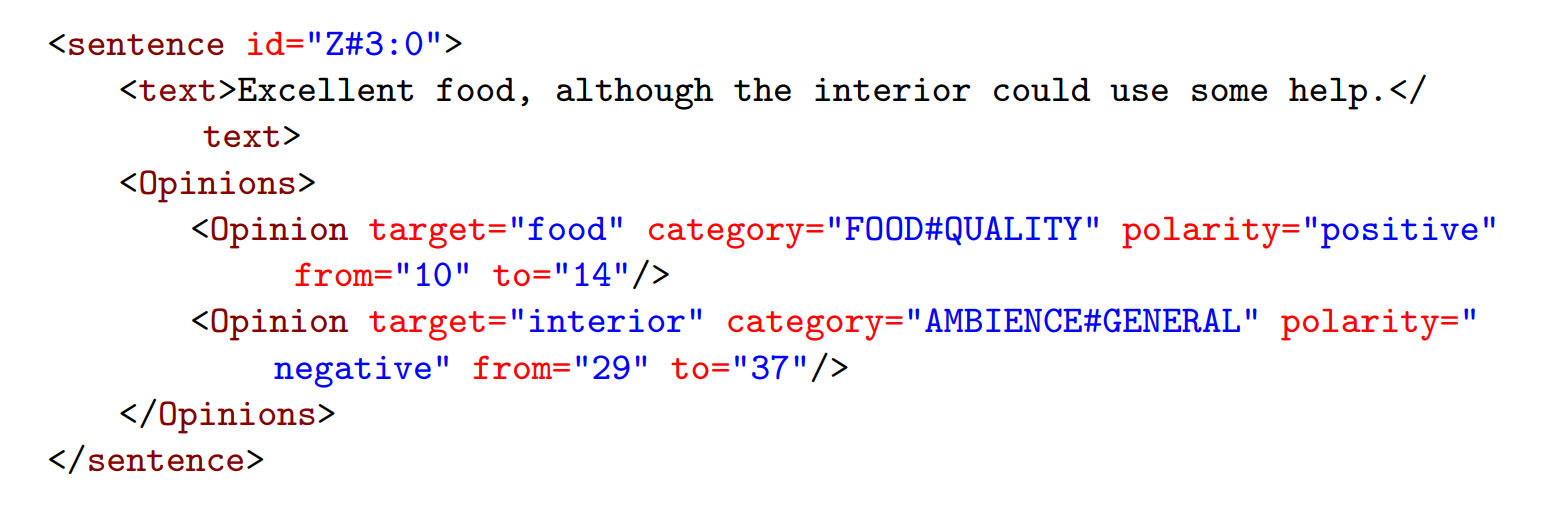
\includegraphics[width=\textwidth]{example_semeval.PNG}
    \caption{A sentence from the SemEval 2016 dataset.}
    \label{fig:example_semeval}
\end{figure}

\section{Training dataset} \label{sec:training}
For our training dataset, we use the Yelp dataset challenge prepared by \textcite{Huang2020JASen} consisting of 17,027 unlabeled review sentences. The original dataset \parencite{Tang2016Yelp} contains much more data attributes. However, only the review text is extracted without any further modification. This dataset is chosen as it resides in the restaurant domain just like our evaluation data. Furthermore, this dataset is much larger compared to the SemEval dataset. While it does not include aspect-level information, it will not be needed due to the unsupervised nature of the model.

%%%%%%%%%%%%%%%%%%%%%%%%%%%%%%%%%%%%%%%%%%%%%%%%%%%%%%%%%%%%%%%%
\chapter{Methodology} \label{chap:methodology}

This chapter explains the models used in this research. First, \cref{sec:formulation} formulates the problem and introduces general notation to the task. Then, \cref{sec:CASC} explains the CASC model in detail. Next, \cref{sec:LCR-Rot} describes the neural model in detail and how it can be injected in CASC.

\section{Task Formulation} \label{sec:formulation}
We formulate the approach as a single-label multi-class classification problem, meaning that the output should can only be one class from multiple classes. Let the input be a corpus $\mathcal{D} = [X_1, X_2, \dots, X_n]$ consisting of $N$ unlabeled review sentences from a domain. Given the set of aspect categories $A$ together with a small list of seed words $L_a$ for each aspect category $a \in A$, and sentiment polarities $S$ along with a small list of seed words $L_s$ for each sentiment polarity $s \in S$. The objective is to predict a pair of $(a, s)$ for a given unseen review sentence.

\section{Modified CASC} \label{sec:CASC}
This section describes the CASC model in detail. It consists of three different stages. In the first step, class vocabularies for aspect and sentiment categories are constructed through contextual embeddings using only seed words. Second, unlabeled data is turned into labeled data in a weakly-supervised manner using overlap scores with the vocabularies from the previous step. Third and last, a simple neural model with a linear layer is implemented to perform ACD and ASC.

\subsection{Class Vocabulary Construction}
With a small set of seed words $L_a$ corresponding to aspect $a \in A$, we find the set of sentences $X_a \subset \mathcal{D}$ which contains any of the seed words. Afterwards, sentence $X_i \in X_a$ is passed to a post-trained Domain Knowledge BERT masked language model (DK-BERT MLM) to predict words for finding replacement candidates of all tokens in the sentence. DK-BERT MLM outputs replacement probability scores $P_i \in \mathbb{R}^{\lvert X_i \rvert \times \lvert V \rvert}$ with V being the vocabulary set used by DK-BERT. However, only replacement candidates of the tokens in the seed words are considered. Next, those replacement candidates are passed through a filter to get rid of stop words and punctuation. Then, the top $K$ words are selected as replacement candidates $R_i$ based on their probability scores computed by DK-BERT MLM. All replacement candidates $R_i$ for all $X_i \in X_a$ are collected and added to a frequency table corresponding to each $a \in A$. Subsequently, the top $M$ most frequent words for aspect category $a$ are selected to construct the aspect vocabulary set $V_a$. Last, words that appear inside multiple vocabularies are removed in both sets. A similar procedure is used to construct the sentiment vocabularies $V_s$ for all $s \in S$.

The intuition behind these steps is that words within a sentence can be replaced by words that carry a similar contextual meaning. DK-BERT MLM is trained to provide such replacement candidates such that the words outputted will resemble the meanings of the seed words closely. Furthermore, the vocabulary sets are disjoint sets to remove ambiguities across aspect and sentiment classes. The filter, which removes stop words and punctuation, further helps the procedure to minimize the overlap between vocabulary sets.

\subsection{Labeled Data Preparation}
Following the work by \textcite{Hu2004Rules}, the CASC model exploits the notion of aspects and opinion terms to be nouns and adjectives or adverbs, respectively. Therefore, nouns, adjectives and adverbs are extracted using a POS tagger as \textit{potential-aspects} and \textit{potential-opinions}. However, we propose a method to extract multiple aspect expressions per sentence instead of a single term.

First, find the set of all sentences $X_q \subset \mathcal{D}$ which contains at least one \textit{potential-aspect} and one \textit{potential-opinion}. Then, sentence $X_j \in X_a$ gets passed through DK-BERT MLM to find replacement candidates with probability scores for each \textit{potential-aspect}. With these replacement candidates, the list $G_{aspect}$ is created by taking top K replacement words based on the probability scores. For sentence $X_j$, we find overlap score $S_a$ of each aspect $a \in A$ by counting the common words between its corresponding aspect vocabulary $V_a$ and the list $G_{aspect}$. Overlap scores for sentences $X_q$ with all aspect categories $A$ are stored in a score matrix $M \in \mathbb{R}^{\lvert X_q \rvert \times \lvert A \rvert}$.

% \todo{Write about averaging vs maximum}

The vocabularies in the previous step were created with DK-BERT which is post-trained using a real-world domain-specific dataset. \textcite{Kumar2021CASC} argue that these datasets are often imbalanced. Some aspect categories appear much less or much more compared than others. This means that the certain vocabularies contain a relatively larger number of semantically coherent words compared to other vocabularies. This difference in quality will affect the variance of the overlap scores per category. Therefore, the overlap scores per category are normalized:

\begin{equation}
    S'_{ja} = \frac{S_{ja} - \mu_{ja}}{\sigma_{ja}},
\end{equation}

\noindent where $S'_{ja}$ is the normalized overlap score of each aspect $a$ corresponding to sentence $X_j$, and $\mu_{ja}$ and $\sigma_{ja}$ are the mean and standard deviations of the overlap scores, respectively, and are computed as follows:

\begin{align}
    \mu_{ja}    & = \frac{1}{\lvert X_q \rvert} \sum_{j=1}^{\lvert X_q \rvert} \mathcal{M}_{ja}, \\
    \sigma_{ja} & = \frac{1}{\lvert X_q \rvert} \sum_{j=1}^{\lvert X_q \rvert} \left ( \mathcal{M}_{ja} - \mu_{ja} \right )^2.
\end{align}

The normalized score $S'_{ja}$ shows how many standard deviations the original score $S_{ja}$ away from the mean value is. For sentence $X_q$, aspect categories are assigned if the normalized score is above a pre-defined threshold $\lambda$. 
% \todo{assumption: one or multiple expression terms for aspect categories?} 
A similar procedure is applied for sentiment categories. With the previous steps completed, a labeled dataset $\mathcal{D}_\mathcal{L} \subset \mathcal{D}$ can be constructed which is a subset of the original corpus.

%%%% Extensions
Building on the original CASC model, the aspect term is extracted in this phase. During the aspect label assignment process, each aspect label $a$ gets an aspect term for each sentence $X$. Similar to the overlap scores, aspects are stored in a matrix. When the aspect label is decided, the corresponding aspect term is assigned to the sentence.

There are multiple ways of assigning aspect. The simplest method would be to assign the noun with the highest overlap score. Another approach could be to identify noun chunks \parencite{Honnibal2020Spacy} and select chunks with the highest averaged overlap scores. 
% \todo{I have not decided what would feasible given the time}

% https://stackoverflow.com/questions/44661200/spacy-to-extract-specific-noun-phrase

\subsection{Joint Neural Network for ACD and ASC} % Basically done
In the original CASC model, the authors used a simple yet effective neural model to classify aspects and sentiment. The authors make use of DK-BERT embeddings and extract the second-to-last hidden layer as embeddings for the tokens in the sentence. Sentences $X_l \in \mathcal{D_\mathcal{L}}$ are represented as $X_l = \left ( [CLS], w_1, \ldots, w_n, [SEP] \right )$, where $w_i$ represents a word in a sentence for $0 \leq i \leq n$. BERT considers the [CLS] and [SEP] as special tokens which denote the start and the end of a sequence, respectively. Therefore, the embeddings of the sequence is $H \in \mathbb{R}^{(n+2) \times d}$ for each token in $X_l$. That means that $d$ is the embedding size of the embedding layer, or in this case, the number of hidden layers in BERT. Afterwards, the global sentence representation $T \in \mathbb{R}^{1 \times d}$ is constructed by averaging embeddings from the non-special tokens: 
\begin{equation} 
    \frac{1}{n} \sum_{i=1}^{n}H_i. 
\end{equation}
Thus, the hidden representations of [CLS] and [SEP] are ignored. Last, the sentence representation $T$ is passed to two different linear layers for ACD and ASC: 
\begin{align}
    \hat{a} & = SoftMax(T \times W_a + b_a), \\
    \hat{s} & = SoftMax(T \times W_s + b_s),
\end{align}
where $W_a \in \mathbb{R}^{d \times \lvert A \rvert}$ and $W_s \in \mathbb{R}^{d \times \lvert S \rvert}$ are trainable weight matrices, and $b_a$ and $b_s$ are the trainable bias vectors. Last, $\hat{a}$ and  $\hat{s}$ denote the probabilities for the aspect category and sentiment polarity.

However, the aspect term positions, extracted during the previous phase, are yet to be exploited in this neural model. Therefore, we suggest to inject the double task LCR-Rot-hop++ model instead of applying the neural model described above. 

\section{Double task LCR-Rot-hop++} \label{sec:LCR-Rot}
This section describes the double task LCR-Rot-hop++ model \parencite{Trusca2020HAABSA++} in detail. This sophisticated model exploits positional information by using three Bidirectional Long Short Term Memory (BiLSTM) layers. Furthermore, two types of attention mechanisms are implemented in a iterative manner to exploit local and global contexts. This model replaces a the third step of of the CASC model described in section \cref{sec:CASC}. The LCR-Rot model was originally solely build for ASC. Therefore, a slight modification will be made to also handle ACD tasks.

Like before, DK-BERT is applied to generate embeddings. Unlike before, sentence $X_l$ is split into the left context, the target, and the right context of lengths $L$, $T$, and $R$, respectively. Moreover, they are represented as $X_l^l = \left ( w_1^l, \ldots, w_L^l \right )$, $X_l^t = \left ( w_1^t, \ldots, w_T^t \right )$, and $X_l^r = \left ( w_1^r, \ldots, w_R^r \right )$, respectively, where $w_i^j$ represent the $i$th word in context $j$. Note that the special tokens are removed. Therefore, the embeddings of a sentence are expressed as $H^l \in \mathbb{R}^{L \times d}$, $H^t \in \mathbb{R}^{T \times d}$, and $H^r \in \mathbb{R}^{R \times d}$. Following, each embedding part is fed to separate BiLSTM layers which produce hidden states $B^l = \left( b_1^l, \dots, b_L^l \right)$, $B^t = \left( b_1^t, \dots, b_T^t \right)$, and $B^r = \left( b_1^r, \dots, b_R^r \right)$. Here, $b_i^j \in \mathbb{R}^{2d}$ represents the hidden state from the $i$th layer of context $j$.

Then, a three-step attention mechanism is iteratively applied over the three hidden states. The first and second mechanisms are rotary attention mechanisms that exploit local information, whereas the third is a hierarchical attention mechanisms which exploits global information. First, new left and right context representations are generated by using old target information. Second, two new target representations are generated by using the context representations produced in first step. Third, the phrase representations are updated by interacting the left and right contexts. The following paragraphs go in mathematical detail.

First, rotary attention mechanisms are applied. The new context representations are a weighted sum of the hidden states of each context: 

\begin{equation}
    r^c = B^{c\top} \times \alpha^c,
\end{equation}

\noindent where $c$ denotes the left or right context of size $C$, $B^c \in \mathbb{R}^{C \times 2d}$ corresponds to the hidden states for context $c$, and $\alpha \in \mathbb{R}^{C}$ denotes the attention weights assigned to each hidden state and is computed by the following function and applying the softmax activation function:

\begin{align}
    \alpha^c                         & = \text{softmax}\left( f \left( B^c, r^t\right) \right), \\
    f \left( B^c, r^t; c, t \right) & = \tanh{\left( B^{c\top} \times W^c \times r^t + b^c \times \mathbf{1} \right)},
\end{align}

\noindent where $t$ denotes the left or right target phrase (distinction is explained in the next step), $r^t \in \mathbb{R}^{2d}$ corresponds to the target representation of target phrase $c$, and $\mathbf{1} \in \mathbb{R}^{C}$ denotes a vector of ones. Then, the trainable parameters are the weight matrix $W_c \in \mathbb{R}^{2d \times 2d}$ and the bias parameter $b_c \in \mathbb{R}$.

In the first iteration, there is no old target information to use. Therefore, the hidden states from the target phrase are averaged by using an average pooling layer resulting in target representation $r^t \in \mathbb{R}^{2d}$. In other iterations, target representations $r^t$ computed in step two are used.

THIS SECTION WILL EXPLAIN THE INNER WORKINGS OF LCR-Rot-hop++. HOWEVER, IT COULD NOT BE FINISHED WITHIN THE PROPOSAL TIME.

% \todo{Write details of HAABSA++}

Modifying this neural model is inspired by the CASC model described above. Instead of passing the sequence representation through a single layer, two similar layers are instantiated for the ACD and ASC tasks. The ASC branch stays identical and the ACD branch is similar to the ASC branch. The only differences are the new weight matrix and bias vector parameter with different dimensionalities.

%%%%%%%%%%%%%%%%%%%%%%%%%%%%%%%%%%%%%%%%%%%%%%%%%%%%%%%%%%%%%%%%
%%%%  The planning chapter will removed after the proposal  %%%%
%%%%%%%%%%%%%%%%%%%%%%%%%%%%%%%%%%%%%%%%%%%%%%%%%%%%%%%%%%%%%%%%

\chapter{Planning} \label{chap:planning}
The figure below shows my rough schedule for the thesis. If time allows, I will tinker with different ATE which is colored light orange. The finishing phase and resit phase are not colored as I do not know what to expect.

\begin{figure}[htbp]
    \centering
    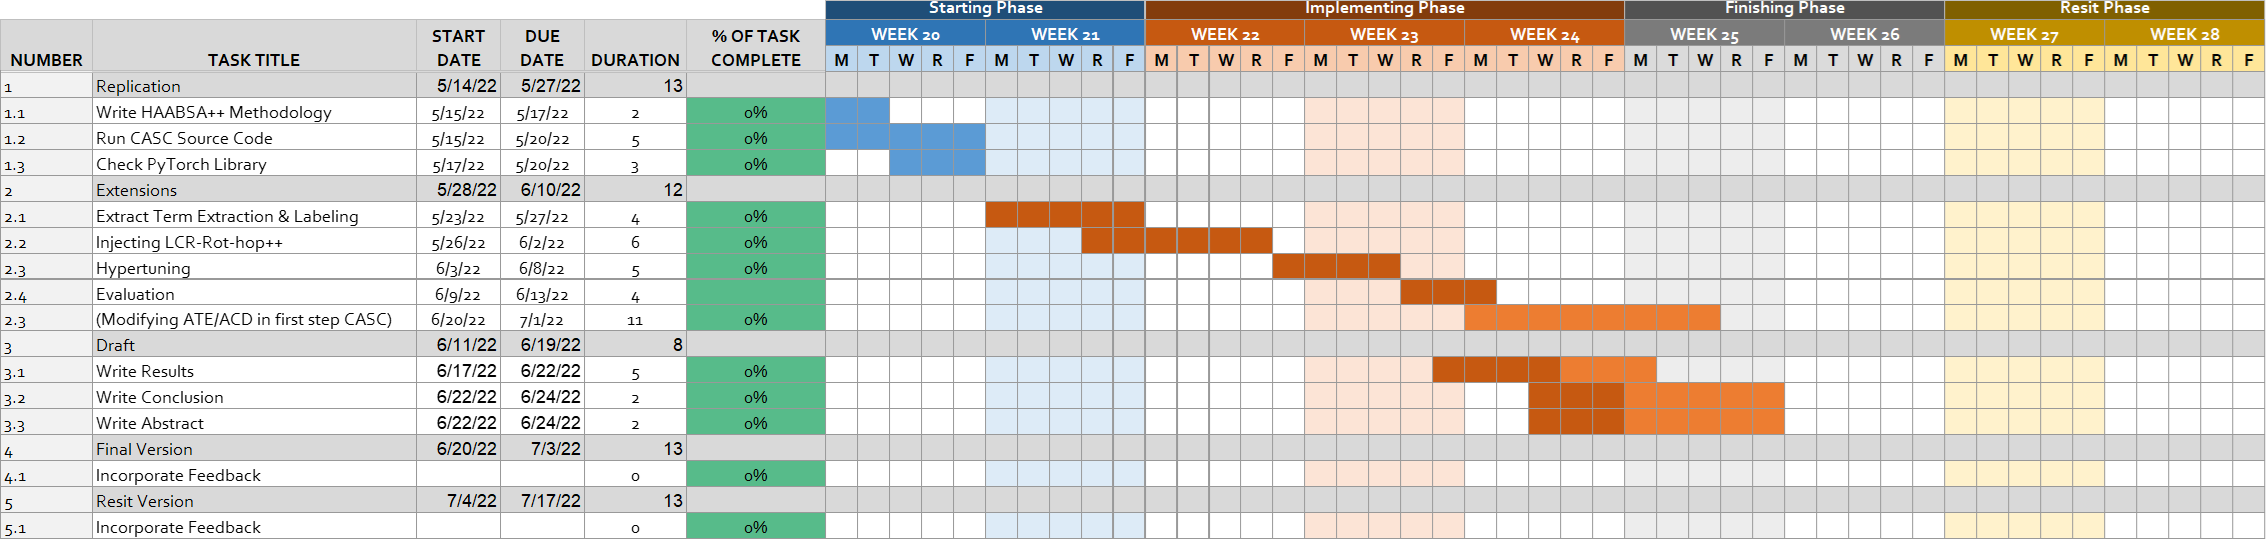
\includegraphics[width=1.5\textwidth, angle=90]{planning_gantt.png}
    \caption{The rough schedule for my thesis}
    \label{fig:planning}
\end{figure}

% \todo[inline]{Unfortunately, I did not have the time to complete the Gantt chart for the thesis timeline. I will still try to make it.}

%%%%%%%%%%%%%%%%%%%%%%%%%%%%%%%%%%%%%%%%%%%%%%%%%%%%%%%%%%%%%%%%
\chapter{Experimental Setup / Results} \label{chap:results}

%%%%%%%%%%%%%%%%%%%%%%%%%%%%%%%%%%%%%%%%%%%%%%%%%%%%%%%%%%%%%%%%
\chapter{Conclusion} \label{chap:conclusion}

\backmatter

% \printbibliography
\bibliographystyle{apalike}
\bibliography{refs}

\appendix


\end{document}
